% !TeX spellcheck = de_CH
\documentclass[
a4paper,
oneside,
10pt,
fleqn,
headsepline,
toc=listofnumbered, 
bibliography=totocnumbered]{scrartcl}

% deutsche Trennmuster etc.
\usepackage[T1]{fontenc}
\usepackage[utf8]{inputenc}
\usepackage[english, ngerman]{babel} % \selectlanguage{english} if  needed
\usepackage{lmodern} % use modern latin fonts

% Custom commands
\newcommand{\AUTHOR}{M. Wieland}
\newcommand{\SECONDAUTHOR}{F. Hauser}
\newcommand{\THIRDAUTHOR}{M. Trentini}
\newcommand{\FOURTHAUTHOR}{P. Scherler}
\newcommand{\INSTITUTE}{Hochschule für Technik Rapperswil}
\newcommand{\LECTURER}{Prof. Dr. Jürg Stadelwieser}
\newcommand{\GITHUB}{https://github.com/michiwieland/businessplan}

% Jede Überschrift 1 auf neuer Seite
\let\stdsection\section
\renewcommand\section{\clearpage\stdsection}

\makeatletter
\newcommand\invisiblesection[1]{%
	\refstepcounter{section}%
	\addcontentsline{toc}{section}{\protect\numberline{\thesection}#1}%
	\sectionmark{#1}\phantom{}}
\makeatother

% Multiple Authors
\usepackage{authblk}

% Include external pdf
\usepackage{pdfpages}

% Layout / Seitenränder
\usepackage{geometry}

% Inhaltsverzeichnis
\usepackage{makeidx} 
\makeindex

\usepackage{url}
\usepackage[pdfborder={0 0 0}]{hyperref}
\usepackage[all]{hypcap}
\usepackage{hyperxmp} % for license metadata

% Glossar und Abkürzungsverzeichnis
\usepackage[acronym,toc,nopostdot]{glossaries}
\glossarystyle{altlisthypergroup}
\usepackage{xparse}
\DeclareDocumentCommand{\newdualentry}{ O{} O{} m m m m } {
	\newglossaryentry{gls-#3}{name={#5},text={#5\glsadd{#3}},
		description={#6},#1
	}
	\makeglossaries
	\newacronym[see={[Siehe:]{gls-#3}},#2]{#3}{#4}{#5\glsadd{gls-#3}}
}
\makeglossaries

% Mathematik
\usepackage{amsmath}
\usepackage{amssymb}
\usepackage{amsfonts}
\usepackage{enumitem}

% Images
\usepackage{graphicx}
\graphicspath{{images/}} % default paths

%figures
\usepackage{tikz}
\usetikzlibrary{shapes.geometric}

%risk-rating
\newcommand\risk[2]{
	\begin{tikzpicture}
	\draw [thick, |->] (0,2) -- (#2,2);
	\draw [fill=red, thick] (#1,2) circle [radius=0.2];
	\end{tikzpicture}
}

% Boxes
\usepackage{fancybox}

%Tables
\usepackage{tabu}
\usepackage{booktabs} % toprule, midrule, bottomrule
\usepackage{array} % for matrix tables

% Multi Columns
\usepackage{multicol}

% Header and footer
\usepackage{scrlayer-scrpage}
\setkomafont{pagehead}{\normalfont}
\setkomafont{pagefoot}{\normalfont}
\automark*{section}
\clearpairofpagestyles
\ihead{\headmark}
\ohead{\TITLE}
\cfoot{\pagemark}

% Pseudocode
\usepackage{algorithm}
\usepackage{algorithmic}

% Code Listings
\usepackage{listings}
\usepackage{color}
\usepackage{beramono}

\definecolor{DarkPurple}{rgb}{0.4, 0.1, 0.4}
\definecolor{DarkCyan}{rgb}{0.0, 0.5, 0.4}
\definecolor{LightLime}{rgb}{0.3, 0.5, 0.4}
\definecolor{Blue}{rgb}{0.0, 0.0, 1.0}

\lstdefinestyle{eclipse-style}{
	language=Java,
	columns=flexible,
	showstringspaces=false,
	basicstyle=\footnotesize\ttfamily, 
	keywordstyle=\bfseries\color{DarkPurple},
	commentstyle=\color{LightLime},
	stringstyle=\color{Blue}, 
	escapeinside={£}{£}, % latex scope within code
	morekeywords={length},
	numbers=left,
	numberstyle=\tiny\color{black},
	frame=single,
}
\lstset{style=eclipse-style}


% Theorems \begin{mytheo}{title}{label}
\usepackage{tcolorbox}
\tcbuselibrary{theorems}
\newtcbtheorem[number within=section]{definiton}{Definition}%
{fonttitle=\bfseries}{def}
\newtcbtheorem[number within=section]{remember}{Merke}%
{fonttitle=\bfseries}{rem}
\newtcbtheorem[number within=section]{hint}{Hinweis}%
{fonttitle=\bfseries}{hnt}

% Dokumentinformationen
\newcommand{\SUBJECT}{Businessplan}
\newcommand{\TITLE}{GitFit}

% pdf metadata
\hypersetup{
	pdfauthor={\AUTHOR},
	pdftitle={\SUBJECT \TITLE}
}

\begin{document}


% German \and
\renewcommand\Authands{ und }
% Front page
\title{\TITLE}
\subject{\SUBJECT}
\author{\SECONDAUTHOR}
\author{\THIRDAUTHOR}
\author{\FOURTHAUTHOR}
\author{\AUTHOR}
\affil{\INSTITUTE}
\affil{\LECTURER}
\date{\today}
\maketitle

\pagecolor{PrimaryColor}\afterpage{\nopagecolor}

\begin{center}
	
\includegraphics[width=0.7\linewidth]{images/front}
\end{center}


\color{black}


% Table of contents
\tableofcontents


% Glossar and acronyms (if included \loadglsentries{glossar})
\printglossary[type=\acronymtype]
\printglossary
\glsaddall


%TODO Total: 20 Seiten -> Es muss ersichtlich sein, was das Produkt bringt.
%TODO Sturktur nach PWC -> Siehe PDF auf Skripte Server


% TODO: Hoher Preis in K.6 wiederspruch zu tiefer Preis in K.2

\clearpage

\section{Management Summary}

\pagestyle{headings}
\pagenumbering{arabic}

Schweizer Fitnesscenter arbeiten heute vorzugsweise mit Stift und Papier, um die Trainingspläne ihrer Kunden zu verwalten. Dies hat einen entscheidenden Nachteil: Die Auswertung ist stark limitiert.

\hfill \\
GitFit ist eine umfassende Lösung für Fitnesscenter, um ihren Kunden ein neuartiges Trainingserlebnis zu bieten. Die Dienstleistung besteht aus einer benutzerfreundlichen App, sowie einer Plattform, über welche sich die teilnehmenden Fitnesscenter austauschen können. Die gesamte Infrastruktur wird von GitFit betrieben. GitFit erlaubt es effiziente und praxisorientierte Trainingspläne zu erstellen und diese komfortable auszuwerten.  
\hfill \\ \\
Die Schweizer Fitnessbranche floriert, gerade durch anhaltenden Trend von einem gesunden und ausgeglichenen Lifestyle. GitFit setzt hier an und liefert ein Produkt, von dem in erster Linie die Fitnesscenter, im Endeffekt aber auch der Endkunde (im weiteren der Sportler genannt) profitiert.  

\hfill \\
Falls die für den Finanzplan getroffenen Annahmen eintreffen, erwarten wir im ersten Geschäftsjahr einen Gewinn von [??]. Dieser wird sich [??] verhalten.


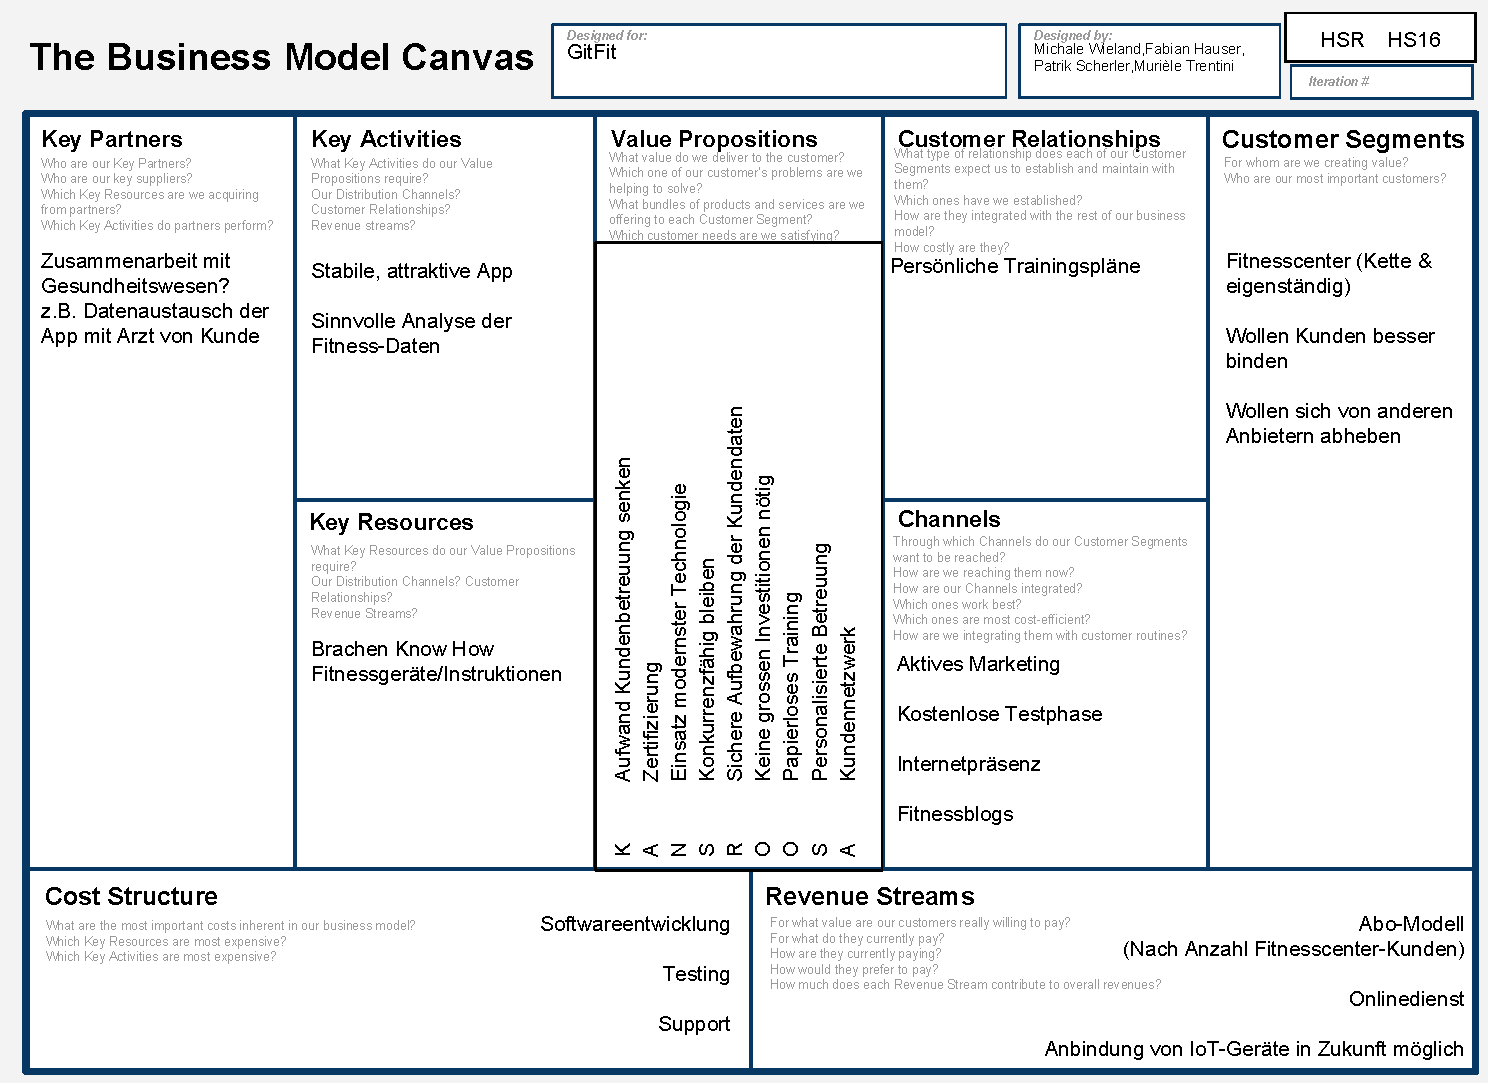
\includepdf[pages=-,addtotoc={1, section, 1, Business Model Canvas, p1},landscape=true]{images/businessmodelcanvas.pdf}
%TODO: Fix title and pdf --> on one page!

\clearpage
\section{Mission, Vision und Strategie: die Zukunft}
\subsection{Mission}
Unsere Aufgabe ist es, vielen Menschen ein völlig neues Erlebnis für ein persönliches Training im Fitnesscenter zu bieten. Wir tun dies, indem wir eine App anbieten, welche die Fitnesslandschaft revolutioniert. Dies zu Preisen, die sich auch kleine Fitnesscenter leisten können.

\subsection{Vision}
Schweizer Fitnesscenter setzen aktuell vorzugsweise auf Papier und Bleistift für die Trainingsplanung ihrer Kunden. Dies ist nicht mehr zeitgemäss und bedarf einer Generalüberholung. Am Puls der Zeit zu sein, bedeutet für ein Fitnesscenter, einen modernen und attraktiven Dienstleister für seine Kunden darzustellen. Die Digitalisierung bietet unendlich viele Möglichkeiten, die es zu nutzen gilt. \\
Wir wollen eine App kreieren, welche die Fitnessbranche wieder auf den aktuellen Stand der Technik katapultiert. Die App bietet aufschlussreiche Statistiken sowie hilfreiche Tipps zur Übung, wenn der Trainer gerade nicht in der Nähe ist.

\subsection{Strategie}
Unser Angebot richtet sich in erster Linie an grosse Fitnesscenter-Ketten, da wir glauben, dass diese an einem übergreifenden Wissensaustausch der Filialen interessiert sind. Im Rahmen der Entwicklung kümmern wir uns in einer ersten Phase um das Anreichern von Stammdaten mit auserwählten Partner-Center. Die Daten sollen als solides und realitätsnahes Fundament für die weitere Entwicklung dienen. In einer zweiten Phase wird dann die App für den Endkunden entwickelt, die ein möglichst komfortables und persönliches Trainingserlebnis vermitteln soll. 

\subsubsection{Wettbewerbsstrategie}
Der Schweizer Fitnessmark boomt und trotzdem ist keine Digitalisierung in der Branche erkennbar. Ähnliche Projekte finden im Ausland bereits Anklang, jedoch gibt es im Inland keine vergleichbare Dienstleistung. Grund genug, diese Lücke zu füllen. Die Schwierigkeit in dem Projekt liegt deshalb weniger in der Positionierung gegenüber ausländischen Dienstleister, sondern vielmehr die heimischen Fitnesscenter mit der neuen Technologie vertraut zu machen.


\clearpage
\section{Produkte und Dienstleistungen: die Marktleistung}

\subsection{Die App}
\begin{figure}[h]
\centering
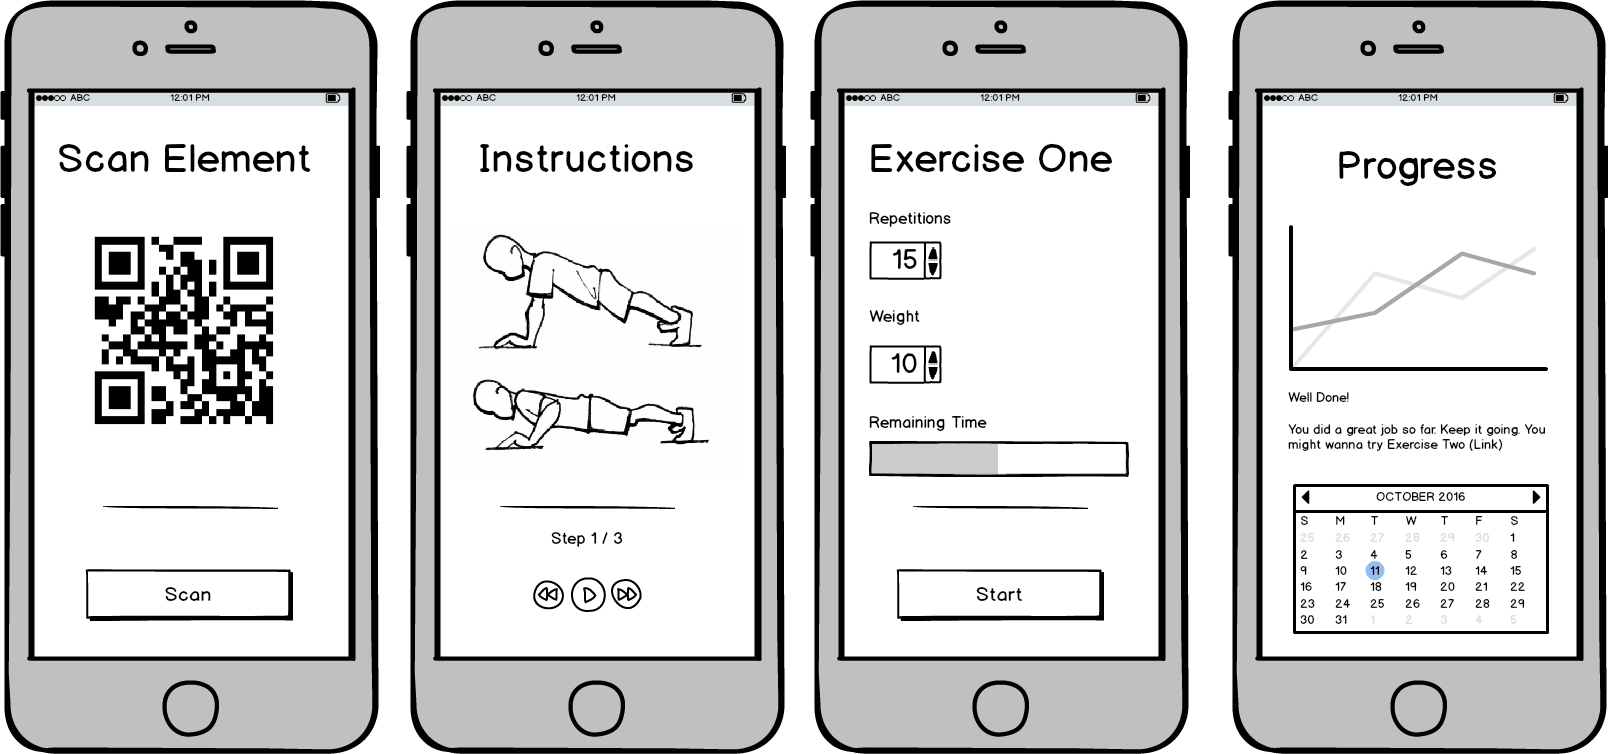
\includegraphics[width=0.5\linewidth]{images/app}
\caption{Wireframe der App}
\label{fig:app}
\end{figure}
Der Kern unseres Angebots bietet die App. In ihr können individuelle Trainingspläne erstellt und Trainingserfolge dokumentiert werden. Übungen können vom Trainer gespeichert und wiederverwendet werden, dadurch lässt sich auch deren Wirksamkeit auswerten. \\ \\
Durch die Verknüpfung mit Activity-Trackern (z.B. Fitness Armbänder) von Drittanbietern hat der Kunde auch stets den Einfluss des Trainings auf den eigenen Körper im Auge. So kann beispielsweise der Verlauf der Herzschlagfrequenz während einer Übung aufgezeichnet werden. \\ \\
Die ausführliche Analysefunktionen bieten Möglichkeiten zur Planung eines Trainings, dass individuell auf den Kunden zugeschnitten ist und seine aktuelle Leistungsfähigkeit und Gesundheit jederzeit berücksichtigt. Es steigert auch die Motivation des Sportlers, da er seine Fortschritte jederzeit betrachten kann. \\ \\
Der Einsatz unseres Produkts würde ein Fitnesscenter zertifizieren und es so von Mitbewerbern abheben.

\subsection{Dienstleistung}
\begin{figure}[H]
	\centering
	\includegraphics[width=0.5\linewidth]{images/GitFit_concept}
	\caption{Übersicht der verschiedenen Akteure}
	\label{fig:GitFit_concept}
\end{figure}
Nebst der App bietet GitFit ein Gesamtsystem in der Cloud, auf das die Fitnesscenter jederzeit Zugriff haben. Kundendaten werden sicher übertragen und in unseren Datencentern gespeichert. Dies garantiert ein hohes Mass an Sicherheit und Verfügbarkeit. Ausserdem können die Daten so von verschiedenen Diensten bearbeitet und ausgewertet werden. \\ \\
Zum einen kann der Betreuer individuelle Trainingspläne für seine Kunden erstellen und hat durch die Analysedaten ein direktes Feedback über deren Trainingserfolge. \\ \\
In Zukunft wäre auch der Einsatz von smarten Fitnessgeräten denkbar, welche sich automatisch (z.B. beim scannen eines QR-Codes) nach dem Trainingsplan des Benutzers einrichten und seine Aktivitäten aufzeichnen.
Zusätzlich könnten so auch Statistiken über die Belegung der Geräte erstellt werden, um Engpässe zu vermeiden. \\ \\
Auch eine Schnittstelle für Hausärzte und Krankenkassen wäre möglich. Beispielsweise um spezialisierte Prämienrabatte anzubieten oder eine bessere Diagnose stellen zu können. \\ \\
Die App für den Endkunden ist gratis. Das Fitnesscenter bezahlt im Abo-Modell, um seine Filiale in der Cloud verfügbar zu machen. Der Preis richtet sich dabei nach der Anzahl Kunden, welche die App nutzen.

\subsection{Kundennutzen}
Darstellung des Kundennutzens mit Helfe des Modells KANSROOSA:
\begin{table}[H]
	\centering
	\begin{tabu} to \linewidth {l l}
		\toprule 
		Bedürfnis & Fitnesscenter \\
		\midrule
		KOMFORT & Aufwand der Kundenbetreuung senken \\
		ANSEHEN & Zertifizierung \\
		NEUHEIT & Einsatz modernster Technologie \\
		SELBSTERHALTUNG & Konkurrenzfähig bleiben \\
		RISIKOLOS & Sichere Aufbewahrung der Kundendaten \\
		ÖKONOMIE & Keine grossen Investitionen nötig \\
		ÖKOLOGIE & Papierloses Training \\
		SYMPATHIE & Personalisierte Betreuung \\
		ANGEHÖRIGKEIT & Kundennetzwerk \\
		\bottomrule 
	\end{tabu} 
	\caption{Anwendung von KANSROOSA an GitFit}
\end{table}


\clearpage
\section{Markt und Kunden: das Zielgebiet}

\subsection{Marktübersicht}

\subsubsection{Marktkapazität / Marktsegmentierung}\label{sec:marktkapazitat}

\paragraph{Fitnesscenter in der Schweiz}
Gemäss einer Studie des BASPO Statistik aus dem Jahre 2014 sind 16\% der Schweizerinnen und Schweizer in einem privaten Fitnesscenter angemeldet \cite{schweizer+fitness}. Damit ist das betreiben eines Fitnesscenters eine lukrative Angelegenheit. In der Schweiz wird die Anzahl auf 700-800 Fitnesscentern im Jahre 2013 geschätzt \cite{fitness-studios+1+milliarde}\cite{fitness+tribune}.

Die meisten Fitnesscenter setzten digitale Mittel lediglich zur Verwaltung des Kundenstammes und Administration ein; nach unseren Recherchen sind weitere Verwaltungsapplikationen bisher nicht im Einsatz.

Unsere Lösung hat grundsätzlich Marktpotential für alle Betreiber von Fitnesscentern, speziell aber in urbanen Gebieten dürfte das Marktvolumen beträchtlich sein. Wir schätzen, dass wir im Optimalfall längerfristig einen Marktanteil von rund 70\% erreichen könnten (ca. 30\% der Fitnesscenter bedient Nischenmärkte).

\paragraph{Grössere Fitnesscenter}
In der Schweiz gibt es einige grössere Anbieter, welche eine Reihe von Fitnesscenter betreiben. Diese sind interessante Abnehmer für unsere Applikation, da diese viele Kunden und damit entsprechende Datenmengen zu verwalten haben.

Die grössten schweizer Fitnesscenter sind\cite{fitness+tribune}:

\begin{multicols}{2}
	\begin{itemize}
		\item \href{http://mfit.ch/}{MFit}
		\item \href{http://www.activfitness.ch/}{ActiveFitness}
		\item \href{http://fitnessconnection.ch/}{FitnessConnection}
		\item \href{http://www.fitnesspark.ch/}{FitnessPark}
		\item \href{http://holmesplace.ch/de/}{Holmesplace}
		\item \href{http://www.kieser-training.com/}{Kieser Training}
		\item \href{http://www.swiss-training.com/}{Swiss Training}
		\item \href{http://tc-training.ch/}{TC Training}
	\end{itemize}
\end{multicols}

\subsubsection{Marktakteure}
In der Schweiz gibt es bisher keine Anbieter von Apps, welche sich direkt an Fitnesscenter wenden. Wir haben uns das schweizer App ''myClubs'' angeschaut, das sich direkt an professionelle Sportler oder Amateursportler wendet.

In Deutschland gibt es einige wenige Anbieter von Apps für den Fitnessgebrauch; die meisten richten sich aber an Sportler und gehen nicht auf Fitnesspläne oder interaktion mit Fitnessgeräten ein. Daneben betreiben ein paar Fitnessketten kleinere Eigenentwicklungen, welche nicht weiter verbreitet sind. Die Firma \emph{eGym} ist ein potentieller direkter Konkurrent.

Mehr Informationen zur potentiellen Konkurrenz sind im Kapitel \ref{sec:konkurrenz-die-mitbewerber} zu finden.


\subsubsection{Erfolgsfaktoren im Markt}

Ein wesentliches Problem von Fitnesscentern ist das halten ihrer Kunden, da inzwischen eine ziemlich ausgebreitete Konkurrenz existiert. Aus diesem Grund werden die Fitnesscenter die App wählen, welche die grösste Kundenbindung ermöglicht. Dabei spielen Design, Qualität und vor allem der gute Ruf eine Rolle.

Wir haben gemäss dem KANSROOSA-Schema in Tabelle \ref{tbl:kundenansprueche-kansroosa} analysiert.
\begin{table}[h]
	\centering
	\begin{tabu}{|l|X|}
		\hline
		Komfort & Weniger Verwaltungsaufwand für das Fitnesscenter \\
		\hline
		Ansehen & Unsere Lösung führt zu einer Moderne und Wissenschaftliche Herangehensweise zur Fitnessplanung\\
		\hline
		Neuheiten & Technisch aktuelle und moderne Lösung; Datenbasierte Fitnesspläne \\
		\hline
		Selbsterhaltung & Vorteile gegenüber der Konkurrenz \\
		\hline
		Risikolos & Durch das Abomodell muss der Kunde keine grossen Risiken eingehen. \\
		\hline
		Oekonomie & Der Einsatz der App bringt potentiell mehr Kunden. \\
		\hline
		Oekologie & Durch den Einsatz einer digitalen Lösung muss kein Papier mehr gedruckt / beschrieben werden. \\
		\hline
		Sympathie & Höhere Kundenbindung durch Personalisierung \\
		\hline
		Angehörigkeit & Der Kunde wird in das Fitness-Netz des Fitnesscenters eingebunden. \\
		\hline
	\end{tabu}
	\label{tbl:kundenansprueche-kansroosa}
	\caption{Kundenansprüche / Erfolgsfaktoren am Markt gemäss KANSROOSA}
\end{table}

\subsubsection{Marktenwicklung}
Der Markt für unsere App ist in den letzten Jahren stark gewachsen \cite{fitness-studios+1+milliarde}\cite{fitness+tribune}, allerdings ist es schwierig, genaue Zahlen zu finden. Zunehmend gibt es auch grössere Fitnessketten (siehe Details im Abschnitt \ref{sec:marktkapazitat}), welche für uns einen interessanten Zielmarkt darstellen.

Aufgrund der beschränkten Zahl Fitnesscenter ist es wichtig, unsere App gut zu profilieren und relativ schnell einen hohen Bekanntheitsgrad zu erlangen.

\subsection{Chancen und Risiken / Nachfrage \& Charakteristika}

Da in der Schweiz erst wenige Fitness-Center im digitalen Zeitalter angekommen sind, gibt es hier eine grosse Chance, Fuss auf dem Markt zu fassen. Einmal etabliert ist es für Konkurrenten schwierig, unser Angebot abzulösen.

Das grösste Risiko geht von der deutschen Konkurrenz aus, da diese aufgrund der finanziellen Gegebenheiten das Produkt zu deutlich günstigeren Preisen anbieten können.


\subsection{Eigene Marktstellung}

Als Startup können wir unsere Firma mit einer neuen Marke auf dem Markt bewegen. Bei den Gründungsmitgliedern ist ein gutes technisches Know-How zur App-Entwicklung vorhanden (Informatik B.sc).

Bisher existieren noch keine über die Bedarfsanalyse herausgehende Geschäftskontakte in diesem Bereich.


\subsubsection{Zielmarkt}

Unser Startup konzentriert sich zum Start auf den Deutsch-Schweizerischen Markt, dies aus administrativen und preispolitischen Gründen, und damit wir uns auf die deutschsprachige Version und damit das grösste schweizerische Marktsegment fokussieren können. Zu einem späteren Zeitpunkt ist die Übersetzung und Ausbreitung des Zielmarktes geplant.

Um das Interesse der Fitnesscenter-Betreiber zu gewinnen, wird unser Verkauf nach der Pilotphase direkt mit den Fitnesscentern in Kontakt stehen. Mehr Informationen zum Verkaufs- und Marketingkonzept sind im Kapitel \ref{sec:marketing-der-weg-zum-markt} ersichtlich.


\clearpage
\section{Konkurrenz: die Mitbewerber}\label{sec:konkurrenz-die-mitbewerber}

Auf dem schweizer Markt ist die Konkurrenz noch eher klein. Erst wenige Fitnesscenter haben sich selber oder wurden von einem Dienstleister digitalisiert. Jedoch gibt es einige Anbieter im nahen Ausland, für welche die Schweiz einen attraktiven Mark bietet. Beide Gruppen wollen wir als potentielle Konkurrenten analysieren.
\subsection{Konkurrenzunternehmen}
\subsubsection{myClubs}\hfill \\
myClubs\cite{myclubs} ist ein schweizer Anbieter einer Fitness App. Ihr Ziel ist es, einem Sportler eine flexible Möglichkeit zu bieten Sport zu treiben. Dabei legen sie ihren Fokus jedoch nicht darauf Fitnesscenter attraktiver zu gestalten oder zu digitalisieren, sondern dem Sportler ein breites Sportangebot in einem einzigen Abo zu bieten. Im Gegensatz zu unserer Strategie, sind die Endkunden von myClub also Sportler, nicht Fitnesscenter.
Das myClubs Angebot umfasst:
\begin{itemize}
	\item Auswahl an verschiedenen Sportarten und -kursen
	\item Auswahl an verschiedenen Partner-Anbietern
	\item Zum Fixpreis im Abosystem
\end{itemize}
Wir heben uns vom Konkurrenten myClub ab, da wir unseren Fokus auf die Verbesserung des Kraft- und Ausdauertrainings in einem Fitnesscenter legen. Dennoch besteht die Möglichkeit, dass ein Fitnesscenter sich dazu entscheidet, ihr Sportangebot bei myClubs anzubieten und dann davon absieht unsere App zu nutzen.
\paragraph{Risikoeinschätzung} \qquad \risk{4}{5} 4/5
\subsubsection{eGym}\hfill \\
Der deutsche Anbieter eGym\cite{egym} verfolgt sehr ähnliche Ziele wie wir. Sie bieten ihren Partnerfitnesscentern eine App mit folgenden Kernfunktionen:
\begin{itemize}
	\item Zugriff auf den Trainingsplan des Fitnesstrainers
	\item Dokumentation von Trainingseinheiten
	\item Kontrolle über Trainingserfolg und Vergleich mit Kollegen
\end{itemize}
eGym wäre ein starker Konkurrent, falls er in den schweizer Markt expandieren würde.
\paragraph{Risikoeinschätzung} \qquad \risk{3}{5} 3/5
\subsubsection{Technogym}\hfill \\
Technogym\cite{technogym}ist ein Anbieter aus der Niederlande. Sie bewegen sich im selben Marktsegment wie wir. Sie verkaufen ihre Fitnessapp sowie angebundene Fitnessgeräte an ihre Fitnesscenter-Kunden.
Ihre Produktpalette umfasst:
\begin{itemize}
	\item Fitnessgeräte mit digitalen Funktionen
	\item vom Trainer erstellte Fitnesspläne mit der Prescribe-App
\end{itemize}
Dabei legen sie ihren Fokus aber vor allem auf den Vertrieb von Fitnessgeräten, wobei wir uns auf die Digitalisierung und das Einbinden der App konzentrieren.
\paragraph{Risikoeinschätzung} \qquad \risk{2}{5} 2/5
\subsubsection{Freeletics}\hfill \\
Der deutsche Dienstleister Freeletics\cite{freeletics} entwickelt eine eigene Fitness-App und betreibt eine Fitnesscenter-Kette.
Folgendes Angebot bietet Freeletics:
\begin{itemize}
	\item App mit Übungsanleitungen und Fortschrittstracking
	\item Ihre eigene Fitnesscenter-Kette
\end{itemize}
Da Freeletics ihre eigene Fitnesscenter-Kette betreibt, wären sie nur dann ein ernsthafter Konkurrent, wenn sie in die Schweiz expandieren und hier ansässige Fitnesscenter vom Markt vertreiben würden.
\paragraph{Risikoeinschätzung} \qquad \risk{2}{5} 2/5
\subsection{Konkurrenzanalyse}
\paragraph{Wie arbeitet die Konkurrenz?} \hfill \\
Passend zum Marktsegment haben alle Konkurrenten eine starke Internet-Präsenz mit ansprechenden, modernen Webseiten. 
Um Junge sportbegeisterte Kunden anzusprechen, setzen sie stark auf social media Marketing über FaceBook, Twitter und Co. Einige betreiben auch einen Blog. Zudem haben sie allgemein eine hohe Medienpräsenz mit Abgabe eines Presse-Kits oder Publi-Reportagen in Zeitschriften. Viele unserer Konkurrenten konzentrieren sich stark auf den Endkunden Sportler.

\begin{figure}[H]
\centering
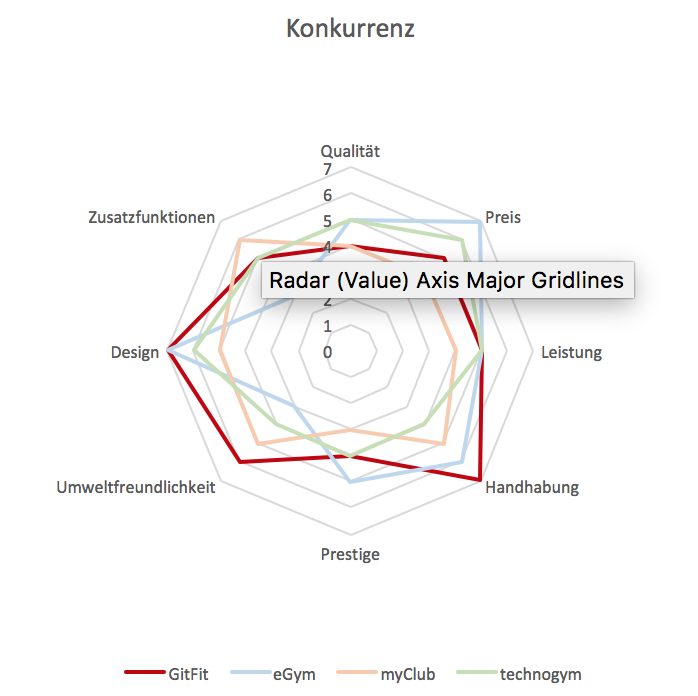
\includegraphics[width=0.9\linewidth]{images/konkurrenz}
\caption{Konkurrenzanalyse}
\label{fig:konkurrenz}
\end{figure}
\paragraph{Konsequenzen}\hfill \\
Aus der Konkurrenzanalyse ergab sich, dass wir uns auf folgende Punkte konzentrieren wollen:
\begin{itemize}
	\item Hoher Preis, dafür sehr gute schweizer Qualität (Label Schweiz)
	\item Modernes Auftreten und Design mit einfacher Handhabung
	\item Wir sprechen direkt Fitnesscenter an und umgehen so den Mittelmann. Dadurch sparen wir wertvolle Ressourcen.
\end{itemize}

\clearpage
\section{Marketing: der Weg zum Markt}\label{sec:marketing-der-weg-zum-markt}

\subsection{Marketingziele}
Um unseren Zielmark zu erreichen, haben wir uns quantitave Ziele gesetzt:
\begin{itemize}
	\item Bis Februar 2017 soll ein Prototyp der App vorgestellt werden können. Dieser ist zwingend um neue Kunden von unserer Idee und den damit verbundenen Vorteilen zu überzeugen.
	\item Bis Mai 2017 ist ein starker Partner gefunden, der im Idealfall über mehrere Fitnesscenter in unterschiedlichen Regionen verfügt.
	\item Bis Ende 2017 ist eine praxisnahe, moderne Trainingsapp entwicket. Die App soll von möglichst vielen Kunden Inputs profitieren und diese benutzerfreundlich digital Abbilden.
	\item Bis Sommer 2018 können mindestens 10 weitere Fintnesscenter mit GitFit ausgerüstet werden.
\end{itemize}

\subsection{Marktpositionierung}
Wir setzen primär auf den Schweizer Mark, wobei wir uns darauf konzentrieren, eine grosse Fitnesscenter-Kette als Partner zu gewinnen. Da die Branche von wenigen ''Big Playern'' dominiert wird,  wird sich deren Einsatz von GitFit bei den Konkurrenzlinien und kleineren Fitnesscenter herumsprechen. Fitnesscenter die noch auf herkömmliche Arbeitsmethoden setzen, werden als nicht mehr zeitgemäss betrachtet und so zu einer Digitalisierung gezwungen. Wir unterscheiden zwischen zwei Typen von Fitnesscenter, die als Kunden in Frage kommen:

\paragraph{Fitnesscenter Ketten} \hfill \\
Die grossen Fitnesscenter-Ketten sind besonders am übergreifenden Wissensaustausch ihrer regionalen Niederlassungen interessiert. So können Trainingspläne von einem Trainer Komitee erstellt werden und national in den verschiedenen Fitnesscenter auf ihre Praktikabilität überprüft werden. Entsprechende Anpassungen wirken sich auf alle beteiligten Fitnesscenter aus. Ebenfalls herrscht eine grosse Konkurrenz zwischen den einzelnen Ketten. Sich abzuheben scheint immer wie schwieriger und deshalb ist GitFit ein willkommenes Produkt zur eigenen Hervorhebung im Markt. 

\paragraph{Kleinere private Fitnesscenter} \hfill \\
Die kleineren, meist privat geführten Fitnesscenter, sind an einer kostengünstigen Lösung interessiert, um nicht an Attraktivität gegenüber den ''Big Playern'' zu verlieren und Schritt zu halten. 


\subsection{Preispolitik}\label{sec:preispolitik}
\subsubsection{Preisfindung}
GitFit wird als Abomodell angeboten, wobei die Abokosten monatlich entrichtet werden müssen. Dies erlaubt es bei insolventen Kunden schnell und unkompliziert die Partnerschaft aufzulösen. Die Kosten werden an der Anzahl an GitFit Accounts in einem Fitnesscenter gemessen. Somit korreliert der Produtkpreis mit der Grösse des Fitnesscenter, weshalb sich auch kleinere Anbieter das Produkt leisten können.

\paragraph{Monatliche Kosten} \hfill
\begin{table}[h]
	\centering
	\begin{tabu} to \linewidth {l r}
		\toprule 
		Beschreibung & Monatliche Abokosten (CHF) \\
		\midrule
		bis zu 200 Kunden & 7.- \\
		ab 200 Kunden & 5.- \\
		\bottomrule 
	\end{tabu} 
	\caption{Preisliste}
\end{table}

\paragraph{Einmalige Fixkosten} \hfill
\begin{table}[h]
	\centering
	\begin{tabu} to \linewidth {l r}
		\toprule 
		Beschreibung & Monatliche Abokosten (CHF) \\
		\midrule
		Sportlerapp & gratis \\
		Trainerapp & gratis \\
		iPad Air 2 für den Trainer (optional) & 400.- \\
		Zugang zu praxiserprobten Trainingspläne (einmalig) & 2750.- \\
		Austattung der Fitnessgeräte mit QR Codes (einmalig) & 500.-  \\
		\midrule
		\textbf{Total (komplettes Paket)} & \textbf{3650.-} \\
		\bottomrule 
	\end{tabu} 
	\caption{Einmalige Fixkosten}
\end{table}

\subsubsection{Rabatte}
Die App basiert auf Praxis erprobten Stammdaten die in einer ersten Phasen mit auserwählten Partnerorganisation aufgebaut werden sollen. Teilnehmende Fitnesscenter profitieren von einer vergünstigten Dienstleistung im ersten Jahr sowie dem Vorteil einer aktiven Mitgestaltung des finalen Produktes. 

\begin{table}[h]
	\centering
	\begin{tabu} to \linewidth {l r}
		\toprule 
		Beschreibung & Fixe Abokosten im ersten Jahr (CHF) \\
		\midrule
		Pro Kunde & 4.50 \\
		\bottomrule 
	\end{tabu} 
	\caption{Preisliste}
\end{table}

\subsubsection{Preisdifferenzierung}
Den Fitnesscenter wird eine umfassende Plattform geboten, mit welcher sie das Verhalten ihrer Kunden vollumfänglich analysieren und auswerten können. Verglichen mit der herkömmlichen Variante mit Stift und Papier, ergeben sie nie dagewesene Möglichkeiten, ohne abstriche in Komfort und Benutzerfreundlichkeit machen zu müssen. Wie in Kapitel \ref{sec:konkurrenz-die-mitbewerber} beschrieben, liegt unser Fokus bei den Fitnesscenter als Endkunde. Dies bedeutet, dass unsere Dienstleistung primär für die Fitnesscenter optimiert sind.

\subsection{Distribution}
Gerade am Anfang des Produkts soll eine enge Bindung zwischen der Entwicklung und den beteiligten Fitnesscentern bestehen. Für die Bekanntmachung unserer Dienstleistung setzen wir auf verschiedenen Distributionspfade. 

\subsubsection{Produktpräsentationen}
Als kleines Startup gehen wir persönlich bei auserwählten Fitnesscentern vorbei und stellen den Nutzen unserer Plattform im persönlichen Gespräch vor. Wir suchen nach einem Partner, der uns auch auf persönlicher und nicht nur finanzieller Ebene entspricht, und unsere Ideologie teilt. Nach einer kurzen, informativen Präsentation hat der potentielle Kunde Zeit, das Produkt live zu testen und zu erleben. Dabei legen wir Wert auf das Hervorheben der Vorteile für das Fitnesscenter und nur zweitrangig für den Endkunden. Insbesordere die Vorteile der statistischen Auswertung müssen dem potentiellen Kuden nach der Präsentation klar sein.

\subsubsection{Internet} 
Mit einem interaktiven und zeitgemässen Webauftritt wollen wir unseren Kunden das Produkt näher bringen. Neue Kunden können sich mit wenigen Klicks für eine Testphase registrierern, worauf der Schritt zum Abo nur noch ein Kleiner ist. Man registriert sich auf der Webseite und bindet den Testaccount an das Fitnesscenter seines Vertrauens. Es soll auch möglich sein, einen GitFit Account zu erstellen ohne bei einem Fitnesscenter angemeldet zu sein. In diesem Fall wird das Fintesscenter in der Region über einen interessierten Kunden informiert. Da die primäre Zielgruppe die Fitnesscenter an sich sind, soll die Webseite auch für diese Zielgruppe interessante Fakten zur Verfügung stellen. So sollen einerseits Erfahrungsberichte anderer Fitnesscenter zu finden sein, sowie einige Beispiele zu den umfassenden Statistiken, die man aus GitFit ziehen kann. Ebenfalls soll es inituitiv logisch sein, mit uns in Kontakt zu treten. Auch die Webseite soll ein Gefühl des "betreut werden" vermitteln.

\subsubsection{Schulungen}
Hat das Produkt im Markt Fuss gefasst, gilt es die Position zu stärken. Dies wird mit motivierten Trainern erledigt, die das Personal des Fitnessstudio für den Einsatz von GitFit schult. Wir bieten ein tägige Kurse an, mit welchen das Personal lern, wie man das volle Potential von GitFit ausnutzen kann.

\clearpage

\subsection{Werbung und Public Relations}
In erster Linie muss ein passendes Fitnesscenter gefunden werden. Dies ist vorzugsweise eine grosse Ketten mit national verteilten Niederlassungen und einem breiten Kundenstamm. Ist ein solches gefunden, kann über den Verband und Krankenkassen gezielt Werbung für das neue Produkt lanciert werden. Ist das Vertrauen einer grossen Kette einmal gewonnen, wird es wesentlich einfacher, dem restlichen Markt unser Produkt vorstellen zu dürfen.

\subsubsection{Angestrebtes Image}
GitFit ist ein innovatives, zukunftsweisendes Startup, das die Fitnessbranche revolutioniert. Fitnesscenter die GitFit unterstützen, werden als modern und attraktiv angesehen. Der Einsatz von GitFit bedeutet für ein Fitnesscenter mehr Kunden, die aus den Möglichkeiten der App, den optimalen Nutzen für ihre Gesundheit ziehen möchten.

\subsubsection{Werbeanstrengungen}
Mit einem prestigeträchtigen Partner lässt sich Werbung vergleichsweise kostengünstig bewältigen. Die grössten Anstrengungen liegen in der Suche eines solchen Partners. Dazu setzen wir uns mit dem Verband der Schweizerischen Fitness- und Gesundheitscenter (SFGV) und den grössten Fitnesscenter-Ketten zusammen. Diesen soll der Nutzen von GitFit vorgeführt werden. Konnte ein Partner gefunden werden, setzen wir bei unseren Werbeanstrengungen insbesondere auf das Internet. Nachdem die Enwicklung an GitFit abgeschlossen ist, werden wir Werbung in Fachzeitschriften schalten. Diese liegen in den Fitnesscenter meist im Empfangsbereich und werden von wartenden Sportler gerne gelesen. Je grösser der Bekanntheitsgrad von GitFit bei den Sportler ist, desto mehr wird das Produkt als notwender Teil eines guten Fitnesscenter gelten. Hat sich der Sportler erst einmal an die Vorzüge der App gewöhnt, möchte er diese nicht mehr missen.

\subsection{Absatzziele}
Ziel ist es, alle grossen Fitnesscenter-Ketten in der Schweiz mit GitFit auszurüsten. Ist dies geschafft, können umfassende Statistiken erstellt werden, die man z.B wieder in die Forschung einfliessen lassen kann und auch für Krankenkassen interessant sein könnten. Natürlich wäre diese Dienstleistung nicht kostenlos und bedarf einer neuen Evaluierung. Da dies aber ein erfolgreiche Platzierung im Mark voraussetzt, wird dieser Schritt hier nicht mehr weiter erörtert.

\clearpage
\section{Beschaffung und Produktion: die Leistungserstellung}
\subsection{Gründung und Hauptsitz}
GitFit wird als GmbH mit Hauptsitz in Cham, ZG gegründet.
\subsection{Beschaffung Arbeitsmaterial}
Unser Bedarf an Material ist zu Beginn sehr begrenzt. Eingekauft werden pro Entwickler ein Notebook zum Programmieren der App und weitere organisatorische Tätigkeiten sowie eine Lizenz für Microsoft Office und Visual Studio. Allfällig benötigte QR-Codes für Fitnessgeräte werden nicht selber produziert, sondern bei einer Druckerei in Auftrag gestellt. Hinzu kommen noch kleine Posten wie Flyer und Visitenkarten.
\subsection{Technologie}
Um unseren Kunden unsere Apps möglichst einfach zugänglich zu machen, setzen wir auf Crossplattform Entwicklung. Dabei nutzen wir die zukunftsträchtige Technologie Xamarin.
\subsection{Personalaufwand}
Im Gründungsjahr umfasst das Team nur die vier Gründungsmitglieder. Geplant ist, das Team in den ersten Geschäftsjahren um ein bis zwei Mitarbeiter zu erweitern.

\clearpage
\section{Management und Organisation: die Köpfe dahinter}

\subsection{Firma}
\begin{tabu} to \linewidth {l X}
	Firmenname & GitFit GmbH \\
	Firmengründer & Muriele Trentini (25\%)  \newline Patrick Scherler (25\%) \newline Fabian Hauser (25\%) \newline Michael Wieland (25\%) \\
\end{tabu} 

\subsection{Rechtsform}
GitFit wird als GmbH in das Handelsregister des Kantons Zug eingetragen. Das Eigenkapital von 20'000 CHF wird von den Teilhaber übernommen.


\subsection{Organisatorisches}
Die Geschäftsleitung wird von Patrick Scherler übernommen. Die vier Gründungsmitglieder haben aber identische Anteile an der Firma und somit auch die gleichen Rechte bei strategischen Entscheiden. Es macht jedoch Sinn, jemanden an die representative Spitze des Unternehmens zu setzen, damit die Rollenverteilung klarer definiert ist.
\begin{figure}[h]
	\centering
	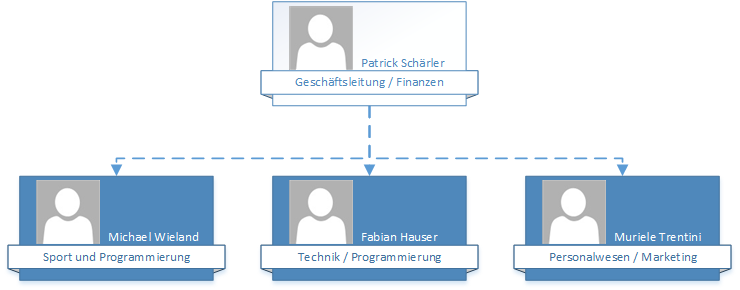
\includegraphics[width=0.9\linewidth]{images/organigramm}
	\caption{Organigramm}
	\label{fig:organigramm}
\end{figure}

\clearpage

\subsection{Das Team}

\subsubsection{Patrick Scherler}
\noindent\begin{minipage}{0.7\textwidth}
	\paragraph{Kontakt} \hfill \\
	Patrick Scherler \\
	<Addr> \\
	<PLZ> <Ort> \\
	<TEL> \\
	
	\paragraph{Funktion} \hfill \\
	Partner, Geschäftsleitung, Entwicklung \\
	
	\paragraph{Ausbildung} \hfill \\
	<JAHR>-<JAHR> \hspace{2cm} <BESCHREIBUNG> \\
		
	\paragraph{Hobbies} \hfill \\
	<HOBBIES> \\
\end{minipage}
\hfill
\begin{minipage}{0.3\textwidth}\raggedright
	
\includegraphics[width=\textwidth]{images/team/pscherler}
\end{minipage}

\subsubsection{Michael Wieland}
\noindent\begin{minipage}{0.7\textwidth}
	\paragraph{Kontakt} \hfill \\
	Michael Wieland \\
	Löwengasse 1 \\
	7208 Malans \\
	079 575 19 18 \\
	
	\paragraph{Funktion} \hfill \\
	Partner, Sport, Marketing, Entwicklung \\
	
	\paragraph{Ausbildung} \hfill \\
	2008-2012 \hspace{2cm} Berufslehre zum Informatiker EFZ \\
	2012-2014 \hspace{2cm} Software Entwickler \\
	2014-2015 \hspace{2cm} Auslandaufenthalt \\
	seit 2015 \hspace{2.2cm} Informatik Studium an der HSR \\
	
	\paragraph{Hobbies} \hfill \\
	Unihockey, Fussball, Fitness, Bass
\end{minipage}
\hfill
\begin{minipage}{0.3\textwidth}\raggedright
	
\includegraphics[width=\textwidth]{images/team/mwieland}
\end{minipage}

\clearpage


\subsubsection{Murièle Trentini}
\noindent\begin{minipage}{0.7\textwidth}
	\paragraph{Kontakt} \hfill \\
	Murièle Trentini \\
	Rickenstrasse 7 \\
	8634 Hombrechtikon \\
	079 603 82 64 \\
	
	\paragraph{Funktion} \hfill \\
	Partner, Personalwesen, Entwicklung \\
	
	\paragraph{Ausbildung} \hfill \\
	2003-2007 \hspace{2cm} MNG Rämibühl: Matura \\
	2010-2013 \hspace{2cm} Biomedizinische Analytikerin HF \\
	seit 2015\hspace{2.3cm} HSR, Informatik Studium\\
	
	\paragraph{Hobbies} \hfill \\
	Segeln, Lesen \\
\end{minipage}
\hfill
\begin{minipage}{0.3\textwidth}\raggedright
	
\includegraphics[width=\textwidth]{images/team/mtrentini}
\end{minipage}

\subsubsection{Fabian Hauser}
\noindent\begin{minipage}{0.7\textwidth}
	\paragraph{Kontakt} \hfill \\
	Fabian Hauser \\
	<Addr> \\
	<PLZ> <Ort> \\
	<TEL> \\
	
	\paragraph{Funktion} \hfill \\
	Partner, Finanzen, Entwicklung \\
	
	\paragraph{Ausbildung} \hfill \\
	<JAHR>-<JAHR> \hspace{2cm} <BESCHREIBUNG> \\
	
	\paragraph{Hobbies} \hfill \\
	<HOBBIES> \\
\end{minipage}
\hfill
\begin{minipage}{0.3\textwidth}\raggedright
	
\includegraphics[width=\textwidth]{images/team/fhauser}
\end{minipage}

\clearpage
\section{Chancen und Risiken: eine ehrliche Bilanz}

\subsection{Risiken}
Nachfolgend sind die wahrscheinlichsten Ereignisse aufgelistet und kurz beschrieben:
\\ \\
\begin{tabu} to \linewidth {l X}
	Wenig Absatz & Unser Produkt stösst auf wenig Begeisterung und wir können nicht genügend Kunden akquirieren. \newline \\
	Keine Grosskunden & Dies ist als separater Punkt aufgeführt, da unsere Strategie das akquirieren von Fitnesscenter-Ketten vorsieht. \newline \\
	Konkurrenz & Das plötzliche Auftauchen eines neuen Mitbewerbers oder die Veränderung einer bestehenden Konkurrenzbeurteilung. \newline \\
	Serverausfall & Das Ausfallen unserer Serverinfrastruktur führt zu einem Unterbruch in der Verfügbarkeit unserer Cloud. \newline \\
	Datendiebstahl & Das mutwillige Entwenden von Kundendaten durch eine Drittperson. \newline \\
	Datenverlust & Der unwiderrufliche Verlust von gespeicherten Kundendaten. \newline \\
\end{tabu}

\hfill \\
In der Tabelle sind die Ereignisse absteigend nach ihrem geschätzten Schadenspotential aufgeführt. Das Risiko entspricht dem Produkt des Schadenspotentials und der Eintrittswahrscheinlichkeit.
\begin{table}[h]
	\centering
	\begin{tabu} to \linewidth {l l l l}
		\toprule
		Ereignis & Schadenspotential & Eintrittswahrscheinlichkeit & Risiko \\
		\midrule
		Wenig Absatz & 4 & 4 & 16 \\
		Keine Grosskunden & 3 & 3 & 9 \\
		Konkurrenz & 3 & 2 & 6 \\
		Serverausfall & 1 & 2 & 2 \\
		Datendiebstahl & 2 & 1 & 2 \\
		Datenverlust & 1 & 1 & 1 \\
		\bottomrule
	\end{tabu}
	\label{tbl:risikoanalyse}
	\caption{Risikoanalyse der wahrscheinlichsten Ereignisse}
\end{table}

Aus den oben berechneten Daten ergibt sich folgendes Diagramm zur einfacheren Risikobeurteilung. Ein Kreis entspricht einem Ereignis und dessen Grösse dem jeweiligen Risiko.
\begin{figure}[H]
	\centering
	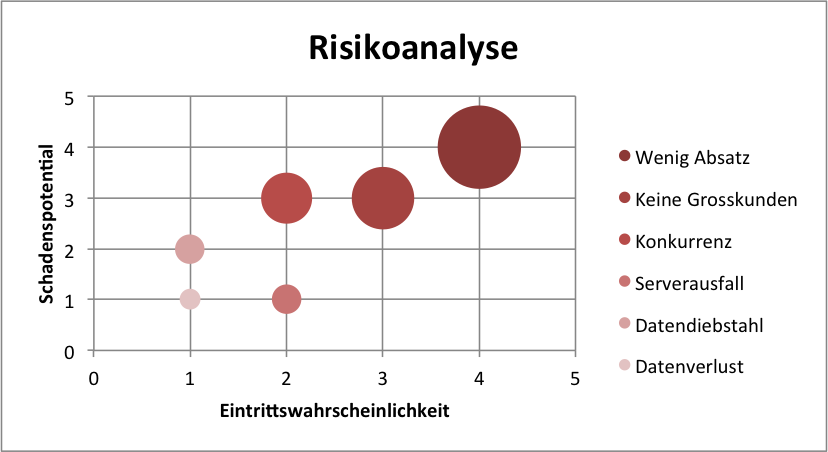
\includegraphics[width=0.5\linewidth]{images/risikoanalyse}
	\caption{Visualisierung der Risikoanalyse}
	\label{fig:visualisierung-risikoanalyse}
\end{figure}

\subsection{Massnahmen}
Zur Reduzierung des Risikos kann entweder das Schadenspotential oder die Eintrittswahrscheinlichkeit verringert werden.
\paragraph{Wenig Absatz}
Das Risiko von zu wenig Absatz ist zwar relativ gross, besteht allerdings fast ausschliesslich zu Beginn der Markteinführung, da unsere Kundenbindung relativ hoch ist. Sobald eine gewisse Menge an Kunden akquiriert ist und daraus Gewinn generiert wird, senkt sich die Eintrittswahrscheinlichkeit beträchtlich. Als Sicherheit sollte hier die Mindestanzahl Kunden berechnet werden, um noch rentabel zu sein. 
\paragraph{Keine Grosskunden}
Das Ausbleiben von Grosskunden wäre ein herber Schlag für unser Unternehmen. Man müsste das Konzept und den Werbeauftritt grundlegend überarbeiten oder die Strategie anpassen und erst auf kleinere Fitnesscenter fokussieren.
\paragraph{Konkurrenz}
Sollte sich die Konkurrenzsituation unerwartet schnell ändern, stellt dies vor allem eine Gefahr dar, solange der Kundenstamm noch relativ klein ist. Eine solide Kundenbasis würde Sicherheit bringen, da die Kundenbindung unseres Produkts eher hoch ist.
\paragraph{Serverausfall, Datendiebstahl und –Verlust}
Das Behandeln dieser Probleme kann durch gängige technische Mittel relativ Einfach umgesetzt werden. Redundante Hardware und regelmässige Datensicherungen Schützen vor längeren Ausfallzeiten und Datenverlust. Verschlüsselung und Sicherheitstechnologien bieten einen Schutz vor Datendiebstählen.

\subsection{SWOT-Analyse}

\clearpage
\section{Finanzieller Teil: die nackten Zahlen}

\subsection{Berechnungsgrundlagen}

\subsubsection{Die Schulungen und Margen auf verkaufte Geräte}
Die durch Schulungen und Margen auf verkaufte Geräte eingenommenen Kosten sind ungefähr linear zu den Einnahmen durch das Abomodell. Wir schätzen diese auf ca. 8\% der Abokosten.
% Und ist damit ca. gleich so gross wie die MwSt - darum ist das im Excel im 3. Jahr nicht eingerechnet.

\subsubsection{Kundenzahlen / Aboumsatz}

Siehe auch Abschnitt \ref{sec:preispolitik} zu den angestrebten Abokosten.

\begin{table}[h]
	\centering
	\begin{tabu} to \linewidth {l X X X}
		\toprule
		Jahr & Fitnesscenter & Mitglieder/Center (im Durchschnitt) & Einnahmen (CHF)\\
		\midrule
		2017 & 3 & 500 & 7500.- \\
		2018 & 30 & 450 & 67'500.- \\
		2019 & 150 & 400 & 300'000.- \\
		\bottomrule
	\end{tabu}
	\label{tbl:kundenzahlen-aboumsatz}
	\caption{Geplante Kundenzahlen / Aboumsatz}
\end{table}

\subsubsection{Die Kosten für das Cloud-Hosting} sind abhängig von der Anzahl verpflichteten Abonnenten; damit skalieren die Kosten gleichmässig mit dem Umsatz, und beträgt ca. 1\% der eingenommenen Abonnementsgebühren.

\subsubsection{Personalkosten}

In den ersten drei Jahren rechnen wir mit den 4 Gründungsmitglieder à 6000.- Brutto (aus betrieblicher Sicht).

\subsubsection{Investoren}

Im ersten Geschäftsjahr müssen Investoren für ca. CHF 500'000 verpflichtet werden, damit die Grundlegenden Entwicklungs- und Expansionskosten der ersten drei Jahre gedeckt sind.

% Doppelte Buchhaltung: heisst aktiva und passiva werden auf zwei verschiedenen Konten verbucht, damit am Schluss der gleiche Betrag herauskommt.
% 
%Bilanz (per Stichtag):
%- Aktiva
%  - Vermögen (Bargeld)
%  - Debitoren (Ausstehende Rechnungen)
%- Materialwert-Abschreibungen
%- Passiva
%  - Kreditor (Schulden)
%  - Aktienkapital
%  - (Gewinn/Verlust)
%-> Bei Aktiva und Passiva muss die gleiche Zahl herauskommen
%
%Erfolgrechne (Periode, zusammenrechnung aus Monaten):
%- Aufwände
%  - Lohnkosten
%  - Miete
%  - Werbung
%
%- Ertrag
%  - Gewinn/Verlust
%  - Verkaufseinnahmen / Dienstleistungen etc.
% Aufwände und Erträge müssen die gleiche Summe haben.


% TODO ZKB KMU Check verwenden
% Das Finanzplanungstool der ZKB muss verwendet werden!
% Investitionsplan für 3 Jahre
% Eröffnungsbilanz + Planbilanzen (3 Jahre) + Planerfolgsrechnungen (3 Jahre) (nur normal case)
% Liquiditätsplan nur für erstes Jahr (pro Monat ausgewiesen)
% Mengengerüst, das den Berechnungen zugrunde liegt.

% TODO Was ist der Kunde bereit zu zahlen?

\clearpage
\section{Umsetzungsplan: die Realisierung}
Musste nicht bearbeitet werden

\clearpage
\appendix

% List of figures
\listoffigures

% List of tables
\listoftables

% Bibliography
\bibliographystyle{plain} 
\bibliography{literatur}

\end{document}